\documentclass[]{article}

\usepackage{amsmath}  % AMS math package
\usepackage{amssymb}  % AMS symbol package
\usepackage{bm}       % bold math
\usepackage{graphicx} % Include figure files
\usepackage{dcolumn}  % Align table columns on decimal point
\usepackage{multirow} % Multirow/column tables
\usepackage{hyperref} % Hyperlinks

\begin{document}

\title{Two-Dimensional Ising Model Simulation:\\with Metropolis Algorithm}% Force line breaks with \\
\author{Tridip Das}
\date{February 18, 2015}% It is always \today, today, but you can specify other dates manually 
\maketitle

\begin{abstract}
This study on Ising model investigates the variation of magnetization with temperature in a ferromagnetic material.
The model try to predict Curie Temperature for a ferromagnetic material with scaled properties. The Monte Carlo simulation with Metropolis algorithm has been
used to predict new spin states by randomly changing spin of a lattice and henceforth trying to minimize the overall energy.
This model also predicts Susceptibility and Specific heat variation with scaled temperature.
\end{abstract}


\section{Introduction} %Title for the section
\label{sec:level1} %Label for the section, to be used for referencing in other parts of the document

The Ising model is a simple representation of the ferromagnetic phase transition at Curie temperature. In this model at low temperature all the lattice site has same spin (say all are up).
The lattice sites preferably occupied by opposite (down) spins with increasing temperature and when it attains Curie temperature the spin distribution goes random in up or down.
The Hamiltonian for Ising model includes only neighbouring site interaction, the long range interaction are neglected. The spin directions may be "Up" (+1) or "Down" (-1).
\begin{equation}
\label{eq:one} %Label for the equation, to be used for referencing in other parts of the document
  H = - J \sum_{<i,j>} S_i S_j
\end{equation}
J is a coupling constant. For ferromagnetic model J $>$ 0. Here it is assumed to be 1.

\section{Monte Carlo Simulation}
In the Ising model, each particle can occupy a site with up or down spin state. In Monte Carlo simulation one site is randomly choose, and the spin state of the particle is reversed.
The acceptance of the new state is determined with application of Metropolis algorithm.

\subsection{Metropolis Algorithm}
The method is a modified Monte Carlo scheme. In this method instead of choosing configuration randomly, configurations are choose with a probability exp(-E/kT) and weight them evenly.
The change in energy is calculated as $\delta E$, if it is $<$ 0, change is accepted. Otherwise, the $\delta E$ with a weighting factor, $e^{-\beta \delta E}$ is compared with a random number $\in [0,1] $ and if the factor is greater, change is accepted.
\\
\subsection{Calculating Observables}
Some quantitative information can be derived from spin array calculations. The magnetization is calculated from spin $\pm 1$ according to below formula:
\begin{equation} 
  m = \frac{1}{N}\sum_{i} \langle S_i \rangle
\end{equation}
\\
The energy, $E$ is calculated as:
\begin{equation} 
  E = - J \sum_{<i,j>} S_i S_j
\end{equation}
i,j are neighbouring lattice position of up, down, left and right.\\
\\
It is also possible to calculate heat capacity, $C_v$ at constant field according to below formula:
\begin{equation} 
  C_v = \frac{\beta}{T}[\langle E^2 \rangle - \langle E \rangle ^2]
\end{equation}
Where, $\beta = \frac{1}{k_B T}$ \\

We can also calculate isothermal susceptibility, $\chi$ with below equation:
\begin{equation} 
  \chi = \beta[\langle M^2 \rangle - \langle M \rangle ^2]
\end{equation}

\section{Results}
The Metropolis based Monte Carlo simulation of Ising model is implemented in Fortran. The code is available in github at \url{https://github.com/tridip66/ising/blob/master/ising.f}, also, other codes can be found in the parent directory, which are used 
to generate the plots.

\subsection{Parameter selection}
The number of iterations to be performed for the magnetization value to reach equilibrium is plotted in figure 1, a magnetization vs temperature curve. In the plot each line corresponds to different number of iterations. It is observed $10^4$ number of iterations is good enough for equilibrium but based on execution time $10^5$ iterations are performed (look into appendix A for details).
\begin{figure}[H]
  \centering
  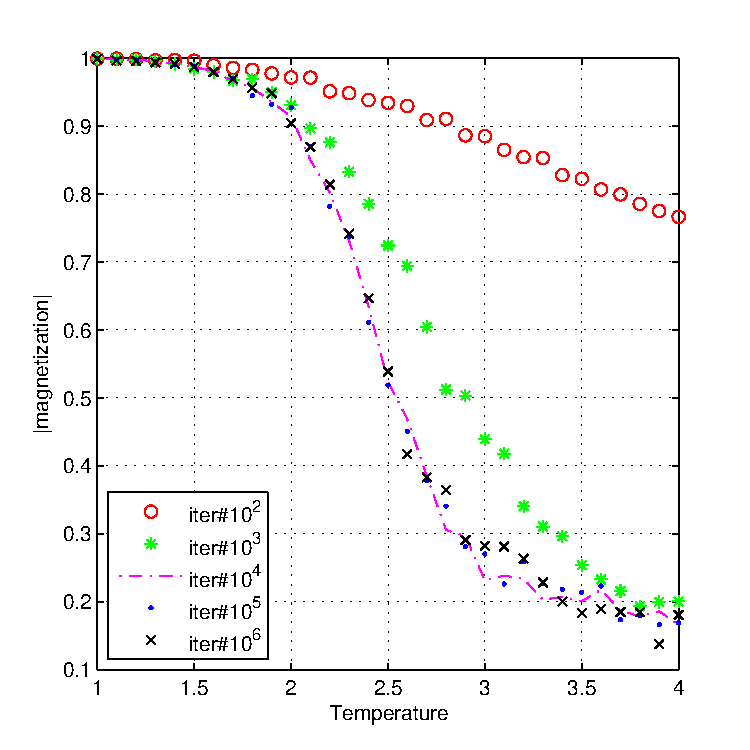
\includegraphics[scale=0.9]{figures/fig_1}% Imports a figure - does not automatically scale
  \caption{\label{fig:epsart} A magnetization vs Temperature plot for different number of iterations performed}
\end{figure}
\\
\\
The lattice site 10x10 is compared with 4x4 and it is observed that 10x10 provides a sharper change in magnetization (figure 3) at Curie temperature. Also, the specific heat and susceptibility change at Curie temperature is not sharp in 4x4 lattice as shown in figure 2.

\begin{figure}[H]
 % \centering
  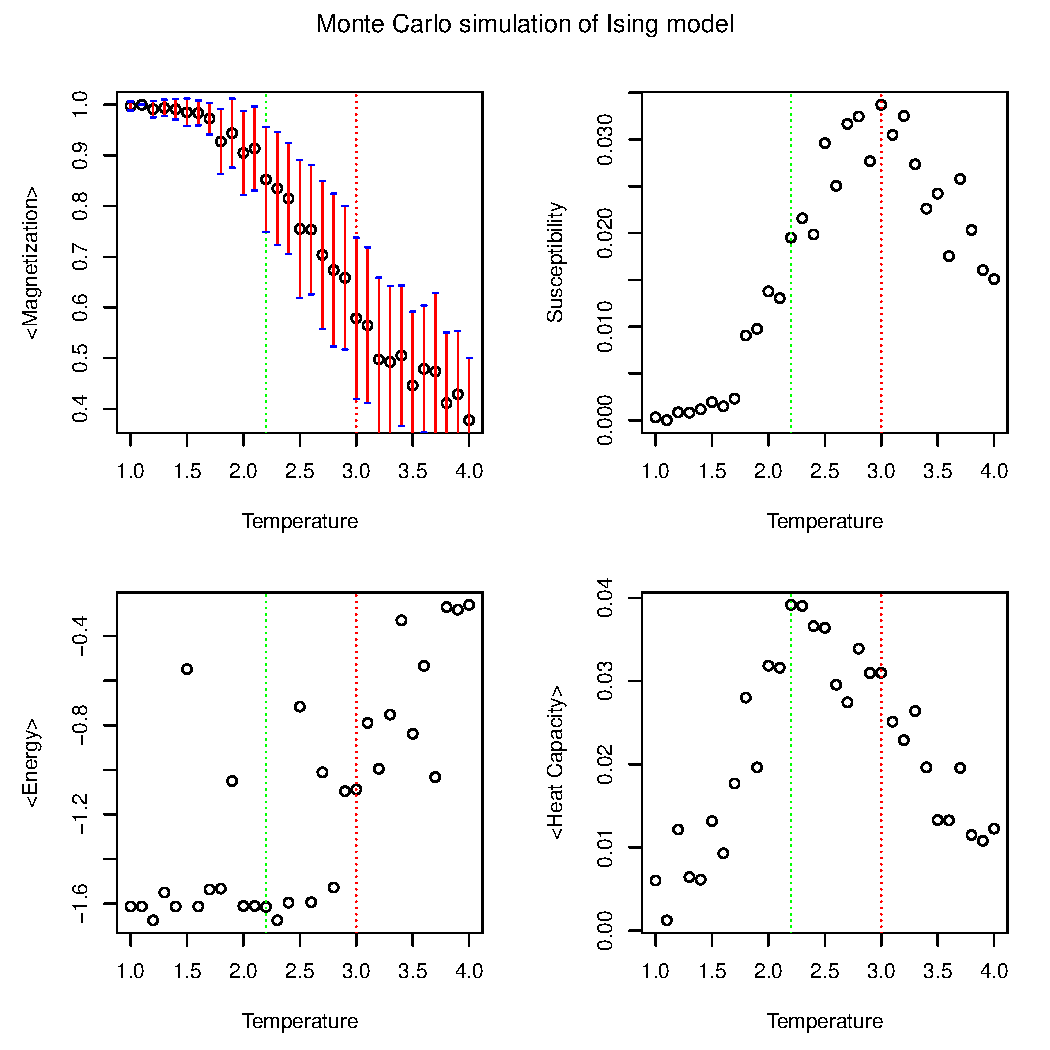
\includegraphics[scale=0.8]{figures/fig_4}% Imports a figure - does not automatically scale
  \caption{\label{fig:epsart} Temperature vs diferent parameters plot for a 4x4 lattice}
\end{figure}

\begin{figure}[H]
  \centering
  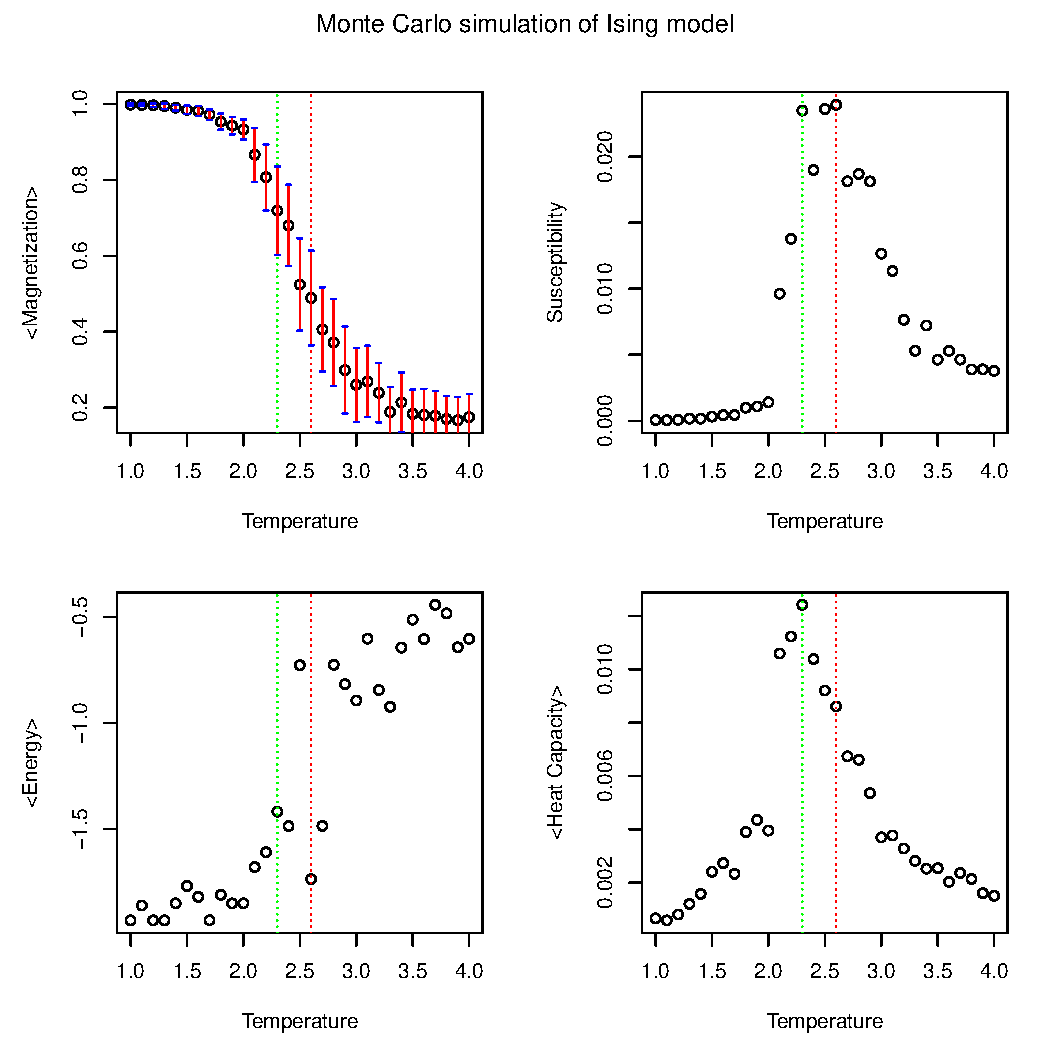
\includegraphics[scale=0.8]{figures/fig_5}% Imports a figure - does not automatically scale
  \caption{\label{fig:epsart} Temperature vs diferent parameters plot for a 10x10 lattice}
\end{figure}

\subsection{Visualization of spin}
A Matlab code, \url{https://github.com/tridip66/ising/spinviz.m} has been developed for visualization of spin states. The figure 4 shows a 10x10 lattice with randomly oriented spins at T=4.
\begin{figure}[H]
  \centering
  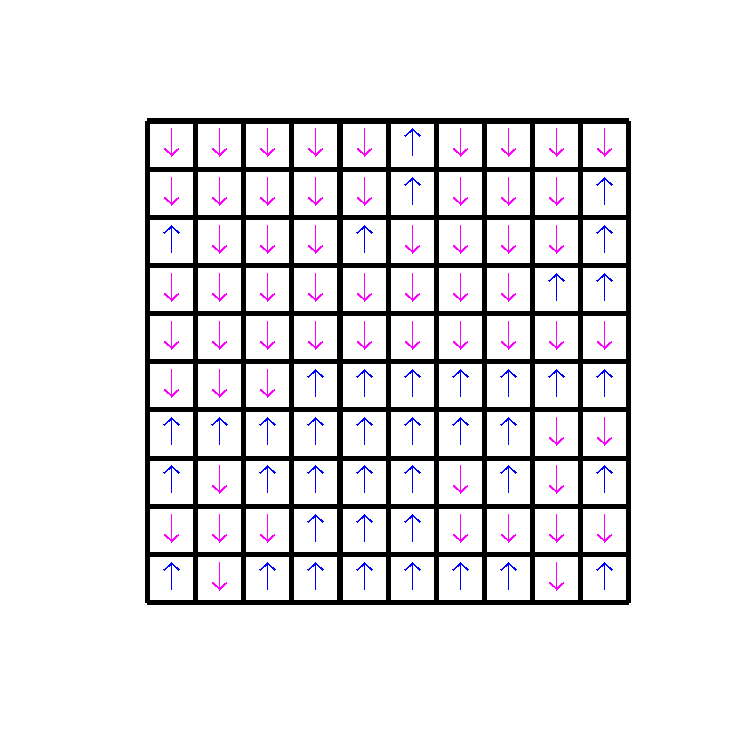
\includegraphics[scale=0.5]{figures/fig_6}% Imports a figure - does not automatically scale
  \caption{\label{fig:epsart} Visualization of spins in a 10x10 lattice at T=4}
\end{figure}
\\
\section*{References}
Charles Kittel and Herbert Kroemer. Thermal Physics. W. H. Freeman, January 1980. 
\\
\url{http://en.wikibooks.org/wiki/LaTeX/Mathematics}
\\
\url{http://en.wikibooks.org/wiki/LaTeX/Importing_Graphics}
\\
\appendix
\section*{Appendix}
Figure 5 shows the iteration time increases linearly with number of iteration as expected. As $10^5$ steps takes around 2 minutes, which is reasonable time with accuracy, so it is selected for further calculations.
\begin{figure}[H]
  \centering
  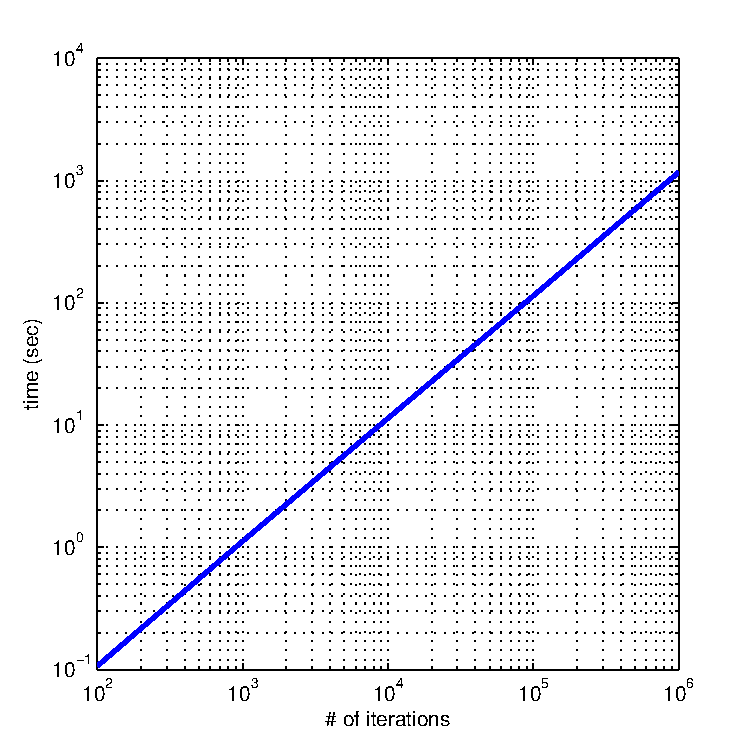
\includegraphics[scale=0.6]{figures/fig_7}% Imports a figure - does not automatically scale
  \caption{\label{fig:epsart} Iteration time vs number of iteration in 10x10 lattice}
\end{figure}

\end{document}
